\documentclass{article}
\usepackage[utf8]{inputenc}
\usepackage{kotex}
\usepackage{graphicx}
\usepackage{subfigure}
\usepackage{caption}
\usepackage{apacite}
\title{PL First Project 20230317}
\author{김승완}
\date{March 2023}

\begin{document}

\maketitle

\section{section1}
안녕하십니까. 저는 홍익대학교 경영학과 4학년에 재학 중인 B831051 김승완입니다. 
\section{section2}
\begin{displaymath}
    -\sum^n_{k=1}k=1+2+3+ \bullet+ \bullet+ \bullet +n=n(n+1)/2
\end{displaymath}
\begin{displaymath}
    -\sum^n_{k=1}k^2=1^2+2^2+3^2+ \bullet + \bullet +\bullet +n^2=n(n+1)(2n+1)/6
\end{displaymath}
\begin{displaymath}
    -\sum^n_{k=1}k^3=1^3+2^3+3^3+ \bullet + \bullet +\bullet + n^3= {n(n+1)}^2
\end{displaymath}
\section{section3}
\begin{figure}
    \centering
    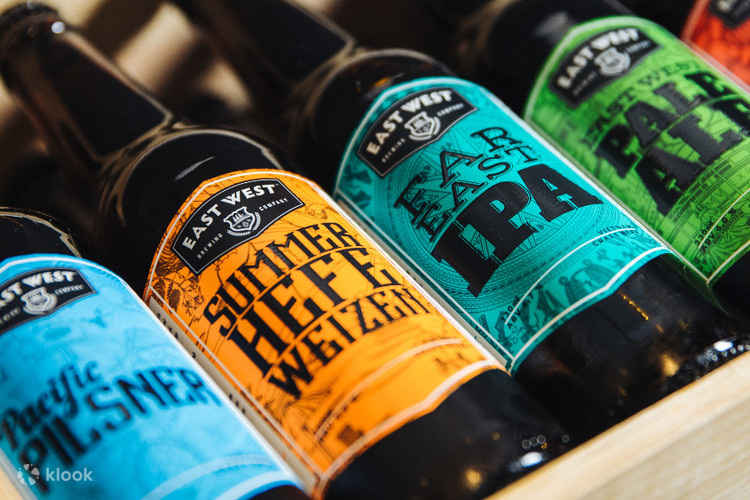
\includegraphics[width=0.45\textwidth]{craftbeer2.jpg}
    \caption{Caption}
    \label{fig:figbeer}
\end{figure}
\subsection{section 3.1}
        Figure \ref{fig:figbeer}은 수제 맥주를 나타냅니다.

\begin{figure}
    \begin{center}
        \subfigure[미나1]{
\includegraphics[width=0.45\textwidth]{mina1.jpg}\label{fig:mina1}}
        \subfigure[미나2]{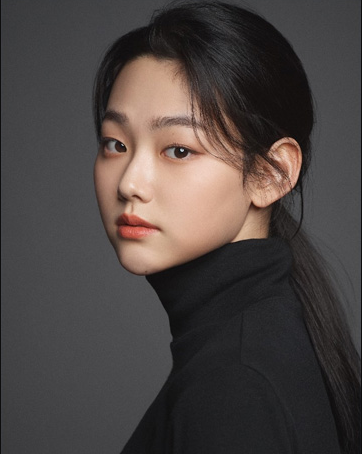
\includegraphics[width=0.47\textwidth]{mina2.png}\label{fig:mina2}}
    \end{center}
\end{figure}
\subsection{section 3.2}
    Figure \ref{fig:mina1}와 \ref{fig:mina2}는 제가 좋아하는 연예인인 강미나입니다.

\section{section4}
본 기고문을 통하여, 저자는 파이썬(Python)이란 언어에 대
하여 소개하고, 이를 공학적 또는 과학적인 분야에서 활용할
수 있는 가능성을 소개하였다. 그러나, 지난 10여년간 오픈소
스 분야에서 괄목한 성장세를 이끌고 있는 파이썬 언어와 이
의 공학적인 활용에 대하여 모든 것을 소개하기에는 지면이
부족할 것이다. 그러나, 최근 산업의 패러다임의 변화가 정형
화된 제조/생산 방식에서 누구나 생산의 주체가 될 수 있는 ‘4
차 산업혁명’시기에 접어들며, 사물인터넷(IoT), 빅데이터(big
data)의 관심이 집중되면서 다양한 기술적, 과학적, 산업적 요
구를 빠르게 반영할 수 있는 새로운 프로그래밍 언어의 요구
는 파이썬과 같이 쉬우면서, 유연하게 다양한 알고리즘을 빠른
시간 안에 구현할 수 있는 언어는 찾아보기 힘들다고 생각된
다. 아두이노와 같은 오픈 소스 하드웨어의 성공을 보면 많은
점을 시사하는데, 그 중에서도 빠른 아이디어의 구현을 가능케
한 점은 매우 높이 평가되고 있는 점이기 때문이다.
저자가 처음으로 파이썬과 Spyder에 관심을 가지는 독자
들에게 입문서로 추천하고픈 문서는 그림 11의 Scipy 강의노
트 모읍집이다.
2011년부터 파이썬의 과학적 활용을 위하여 python,
Numpy, Scipy, 그리고 matplotlib에 대한 기초 설명과, 활용법에 대하여 정리한 자료를 배포하고 있다. 제목은 강의노트
이지만, 몇몇의 편집자가 이를 다듬어서 입문서로 각색한 자
료로 충분히 도서로서 활용이 가능하다.
공학분야에서의 프로그래밍 언어의 필요성은 두말할 필요
가 없다. 하드웨어와 시스템 펌웨어 수준의 저수준에서의 제
어 프로그래밍도 필요하고, 운영체계위에서 데이터 네트워크
레벨에서의 고수준의 제어 및 데이터 처리 알고리즘도 필요하
다. 그러나, 이 모든 레벨의 수준에서 다양한 프로그래밍 언어
를 이해하고 섭렵하여 활용하는 것은 매우 많은 시간과 노력
을 필요로 하는 일이다. 그런 의미에서 파이썬(Python) 언어
는 앞에서 언급한 그런 필요성들을 어느 정도는 만족할 수 있
는 언어일 것이다. 아직 국내에서는 파이썬을 공학적으로 이,
용하는 사례들이 많지는 않지만, 많은 미국의 대학에서 교육
적인 목적으로 파이썬을 활용하고 있으며, 구글과 같은 성공
모델을 기반으로 지속적으로 파이썬의 활용이 확산되어 나갈
것으로 사료된다. \cite{lee2016공학적}.
\bibliographystyle{apacite}
\bibliography{hw0}

\end{document}

